\chapter{Frequency Modulated Continuous Wave Radar}
As the name Frequency Modulated Continuous Wave (FMCW) implies, a FMCW radar is
a continuous time system which transmits and receives a periodic signal whose 
frequency has been modulated. As a periodic signal, the transmitted signal has
the complex form (with unit-normalized amplitude)
\begin{equation}
	\label{eq:complex-sinusoid}
	p(t) = e^{j2\pi f(t)t}.
\end{equation}
The typical frequency modulation used in FMCW radar systems is the sawtooth
modulation, given by
\cite{iovescufundamentals, wang2008digital}
\begin{equation}
	\label{eq:sawtooth}
	f(t) = f_c + \alpha (t - kT_c), \quad\text{for } kT_c \leq t < (k+1)T_c, \quad
	k \in \mathbb{Z}
\end{equation}
where $\alpha > 0$ is the chirp-rate  $\frac{df}{dt}$, $f_c$ is the base
carrier frequency (e.g. 77 GHz), and $T_c$ is the period of the chirp. To
simplify the calculations, we will deal with a single chirp until for range
calculations, thus the frequency for a single chirp is 
\begin{equation}
	f(t) = f_c + \alpha t \quad\text{for } 0\leq t < T_c.
\end{equation}

The maximum frequency of each chirp is 
\begin{equation}
	f_{max} \triangleq f_c + \alpha T_c,
\end{equation}
and the bandwidth $B$ of the signal is
\begin{equation}
	B = f_{max} - f_c = \alpha T_c.
\end{equation}

Combining the sawtooth frequency modulation (\ref{eq:sawtooth}) with the complex
sinusoid (\ref{eq:complex-sinusoid}), we get
the transmitted (TX) signal as
\begin{equation}
	p(t) = e^{j(2\pi f_c t+ \pi \alpha t^2)}.
\end{equation}

\begin{figure}[h]
	\centering
	\begin{subfigure}[b]{0.8\textwidth}
		\begin{tikzpicture}
			\begin{axis}[
			axis x line = bottom,
			axis y line = left,
			xlabel = $t$,
			ylabel=$f(t)$,
			xmin=0, xmax=8,
			ymin=0, ymax=3.2,
			xtick=\empty,
			ytick=\empty,
			xlabel near ticks,
			ylabel near ticks,
			extra x ticks={4,8},
			extra x tick labels={$T_c$, $2T_c$},
			extra y ticks={0, 1, 3},
			extra y tick labels={$0$, $f_c$, $f_{max}$},
			]
			\draw 
				(axis cs:1.5, 1.75)
				-| (axis cs:2, 2)
				node [near end, right]
				{$\alpha$};
			\addplot [
			domain=0:8,
			samples=100,
			color=black,
			]
			{(1 + 0.5*x)*(x<4)+(1+0.5*(x-4))*(x>4)};
			\end{axis}
		\end{tikzpicture}
		\label{fig:sawtooth}
		\caption{Example of sawtooth frequency modulation}
	\end{subfigure}
	\begin{subfigure}[b]{0.8\textwidth}
		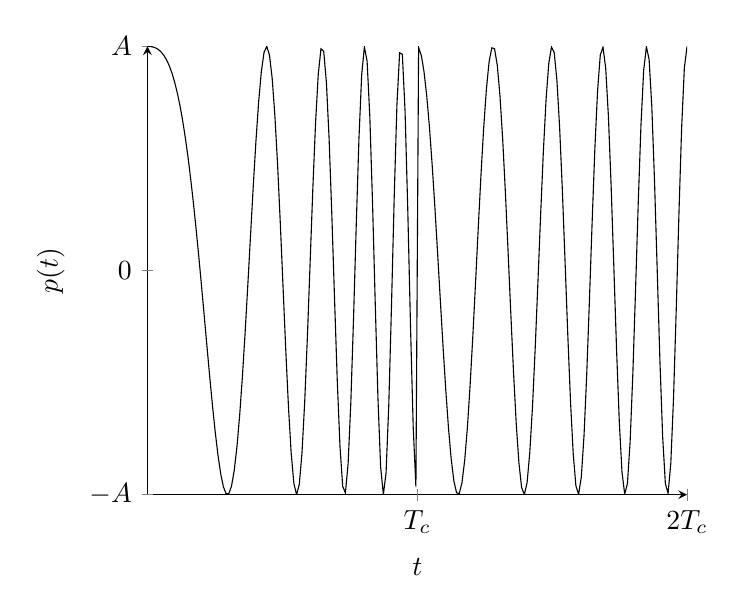
\begin{tikzpicture}
			\begin{axis}[
			axis x line = bottom,
			axis y line = left,
			xlabel = $t$,
			ylabel=$p(t)$,
			xmin=0, xmax=8,
			ymin=-1, ymax=1,
			xtick=\empty,
			ytick=\empty,
			xlabel near ticks,
			ylabel near ticks,
			extra x ticks={4,8},
			extra x tick labels={$T_c$, $2T_c$},
			extra y ticks={-1, 0, 1},
			extra y tick labels={$-A$, $0$, $A$},
			]
			\addplot [
			domain=0:8,
			samples=200,
			color=black,
			]
			{cos(deg(2*pi*((0.125 + 0.25*x)*(x<4)+(0.25+0.125*(x-4))*(x>4))*x)};
			\end{axis}
		\end{tikzpicture}
		\label{fig:pulse}
		\caption{Example of TX signal $p(t)$}
	\end{subfigure}
\end{figure}

\section{Range Measurement}
\label{sec:range}
Consider a target at a distance $d$ from the radar, such that the transmitted
(RX) signal reflects off the target and returns to the radar. This received signal
will be a time delayed version of the TX signal, where the time delay $\tau$ is
given by
\begin{equation}
	\tau = \frac{2d}{c}
\end{equation}
where $c$ is the speed of light. The RX signal thus has the form
\begin{equation}
	p(t-\tau)=e^{j(2\pi f_c (t-\tau) + \pi\alpha (t-\tau)^2)}.
\end{equation}

\begin{figure}[h]
	\centering
	\begin{tikzpicture}
		\begin{axis}[
		axis x line = bottom,
		axis y line = left,
		xlabel = $t$,
		ylabel=$f(t)$,
		xmin=0, xmax=8,
		ymin=0, ymax=3.2,
		xtick=\empty,
		ytick=\empty,
		xlabel near ticks,
		ylabel near ticks,
		extra x ticks={1,4,8},
		extra x tick labels={$\tau$,$T_c$, $2T_c$},
		extra y ticks={0, 1, 1.5, 3},
		extra y tick labels={$0$, $f_c$, $f_b$, $f_{max}$},
		]
		\draw[dashed] (axis cs:0, 1.5) -| (axis cs:1, 0);
			
		\addplot [
		domain=0:8,
		samples=100,
		color=black,
		]
		{(1 + 0.5*x)*(x<4)+(1+0.5*(x-4))*(x>4)};
		\addplot [
		domain=0:8,
		samples=100,
		color=red,
		]
		{(x<1)*1 + (1+0.5*(x-1))*(x>1)*(x<5) + (1+0.5*(x-5))*(x>5)};
		\end{axis}
	\end{tikzpicture}
	\label{fig:received}
	\caption{Frequency of RX signal (delayed by time $\tau$)}
\end{figure}

To recover $\tau$, and subsequently $d$, we define a new dechirped signal $r(t)$
as the product of the transmitted signal with the complex conjugate of the
received signal
\begin{align}
	r(t) &\triangleq p(t)p^*(t-\tau) \\
	&= e^{j(2\pi f_c t + \pi \alpha t^2)}e^{-j[2\pi f_c (t-\tau) + \pi\alpha (t-\tau)^2 ]} \\
	&= e^{j(2\pi f_c \tau - \pi \alpha \tau^2)}e^{j2\pi\alpha\tau t}.\label{eq:range}
\end{align}
Note, the first exponential in (\ref{eq:range}) only depends on $\tau$, so it is
a constant phase term. However, the second term varies according to a constant
frequency (named the beat frequency) $f_b$
\begin{equation}
	f_b \triangleq \alpha \tau.
\end{equation}
The maximum beat frequency occurs when $\tau = T_c$, as any $\tau \in (T_c, 2T_c]$ will
appear as $\tau^*$
\begin{equation}
	\tau^* = \tau - T_c, \quad \tau \in (T_c, 2T_c]
\end{equation}
and thus the recovered distance $d^*$ will be less than the true range the
target is from the radar. From this, we can get our maximum recoverable distance
for a given chirp period
\begin{equation}
	d_{max} = \frac{c T_c}{2}.
\end{equation}
To recover the beat frequency $f_b$ from the dechirped signal, $r(t)$, we can
simply use the Fourier Transform to get
\begin{align}
	R_r(f) &= \int_{-\infty}^{\infty} r(t) e^{-j2 \pi ft} dt\\
	&= \int_{-\infty}^{\infty} e^{j(2\pi f_c \tau - \pi \alpha \tau^2)}e^{j2\pi\alpha\tau t} e^{-j2\pi ft}dt\\
	&= e^{j(2\pi f_c \tau - \pi \alpha
	\tau^2)}\int_{-\infty}^{\infty}e^{-j2\pi(f - \alpha\tau ) t} dt\\
	&= e^{j(2\pi f_c \tau - \pi \alpha \tau^2)}\delta (f - \alpha \tau),
\end{align}
where $\delta(f)$ is the Dirac Delta function.

Now consider the case of multiple ($N$) objects at different distances $d_i$ from the radar.
\begin{equation}
	d_i \not = d_j \quad \text{for } i \not = j, \quad i,j \in [1, N]
\end{equation}
Each of these objects will reflect the transmitted chirp with a unique delay
$\tau_i$, and therefore will have a unique beat frequency corresponding to these
delays. Using the continuous time Fourier Transform, we can always resolve the
unique beat frequencies corresponding to the time delays. In practice, there is
a limit to the range resolution as a result of sampling the received signals,
which will be discussed in Chapter 3.

\begin{figure}[h]
	\centering
	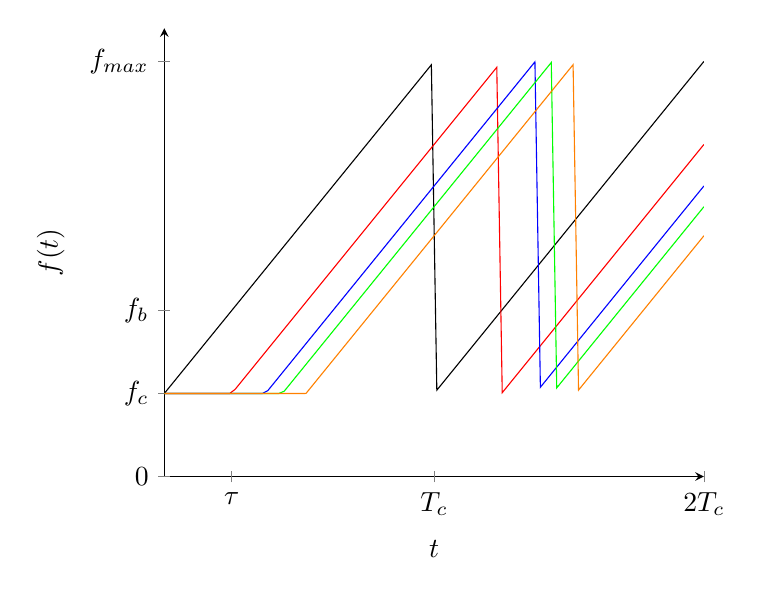
\begin{tikzpicture}
		\begin{axis}[
		axis x line = bottom,
		axis y line = left,
		xlabel = $t$,
		ylabel=$f(t)$,
		xmin=0, xmax=8,
		ymin=0.5, ymax=3.2,
		xtick=\empty,
		ytick=\empty,
		xlabel near ticks,
		ylabel near ticks,
		extra x ticks={1,4,8},
		extra x tick labels={$\tau$,$T_c$, $2T_c$},
		extra y ticks={0.5, 1, 1.5, 3},
		extra y tick labels={$0$, $f_c$, $f_b$, $f_{max}$},
		]
		\addplot [
		domain=0:8,
		samples=100,
		color=black,
		]
		{(1 + 0.5*x)*(x<4)+(1+0.5*(x-4))*(x>4)};
		\addplot [
		domain=0:8,
		samples=100,
		color=red,
		]
		{(x<1)*1 + (1+0.5*(x-1))*(x>1)*(x<5) + (1+0.5*(x-5))*(x>5)};
		\addplot [
		domain=0:8,
		samples=100,
		color=blue,
		]
		{(x<1.5)*1 + (1+0.5*(x-1.5))*(x>1.5)*(x<5.5) +
			(1+0.5*(x-5.5))*(x>5.5)};
		\addplot [
		domain=0:8,
		samples=100,
		color=green,
		]
		{(x<1.75)*1 + (1+0.5*(x-1.75))*(x>1.75)*(x<5.75) +
			(1+0.5*(x-5.75))*(x>5.75)};
		\addplot [
		domain=0:8,
		samples=100,
		color=orange,
		]
		{(x<2.1)*1 + (1+0.5*(x-2.1))*(x>2.1)*(x<6.1) +
			(1+0.5*(x-6.1))*(x>6.1)};
		\end{axis}
	\end{tikzpicture}
	\label{fig:received}
	\caption{Frequencies of reflected signals from multiple objects}
\end{figure}

\section{Velocity Measurements}
To determine the velocity of an object, we can compare the phases of two chirps
reflected from the moving object. Recall from (\ref{eq:range}) that the first
exponential term in $r(t)$ has no dependence on $t$, so it fully describes the phase. We
can approximate this phase as a linear function of the time delay $\tau$, 
\begin{align}
	\phi(r(t)) &= 2\pi f_c \tau - \pi \alpha \tau^2 + 2\pi\alpha\tau t \\
	\implies \angle r(t) &\approx 2\pi f_c \tau.
\end{align}
For an object moving with velocity $v$ and initial range $d_0$, the time delay
$\tau$ is given by 
\begin{equation}
	\tau = \frac{2(d_0 + vt)}{c}, \label{eq:moving-tau}
\end{equation}
so the linear phase approximation becomes
\begin{equation}
	\phi(r(t)) \approx \frac{4\pi(d_0 + vt)}{\lambda},
\end{equation}
where $\lambda = \frac{c}{f_c}$ the wavelength of
the carrier signal. Now, the phase difference $\Delta \phi$ between two
dechirped signals separated by
$T_c$ is
\begin{equation}
	\Delta\phi = \frac{4\pi \Delta d}{\lambda},
\end{equation}
where $\Delta d$ is the distance the object travels over $T_c$ between the two
chirps. For an object traveling at a velocity $v$, this distance is
\begin{equation}
	\Delta d = v T_c, 
\end{equation}
so the phase difference becomes
\begin{equation}
	\label{phase_diff}
	\Delta\phi = \frac{4\pi v T_c}{\lambda}.
\end{equation}
However, phase difference is inherently ambiguous unless $|\Delta\phi|<\pi$, so
we find the maximum velocity measurable by two chirps spaced $T_c$ apart is
given by
\begin{equation}
	v_{max} = \frac{\lambda}{4 T_c}.
\end{equation} 

This two-chirp approach fails if we have multiple objects moving with different
velocities, but the same range at the time of measurement. The reflected chirps
will produce idential beat frequencies in this scenario, so the range processing
Fourier Transform will result in a single peak representing the combined signals
from the equidistant objects. In this case, we can use $K$ equally spaced chirps 
transmitted by the radar over a chirp frame $T_f = KT_c$. 

\begin{figure}[h]
	\centering
	\begin{tikzpicture}
		\begin{axis}[
		axis x line = bottom,
		axis y line = left,
		xlabel = $t$,
		ylabel=$f(t)$,
		xmin=0, xmax=8.5,
		ymin=0.5, ymax=5.2,
		xtick=\empty,
		ytick=\empty,
		xlabel near ticks,
		ylabel near ticks,
		extra x ticks={2,4,8},
		extra x tick labels={$T_c$, $2T_c$, $T_f =
			KT_c$},
		extra y ticks={0.5, 1, 5},
		extra y tick labels={$0$, $f_c$, $f_{max}$},
		]
		\addplot [
		domain=0:8,
		samples=100,
		color=black,
		]
		{(1 + 2*x)*(x<2) + (1+2*(x-2))*(x>2)*(x<4) + (1+2*(x-4))*(x>4)*(x<6) + (1+2*(x-6))*(x>6)*(x<8)};
		\end{axis}
	\end{tikzpicture}
	\label{fig:chirp-frame}
	\caption{Chirp frame $T_f$ consisting of $K$ chirps}
\end{figure}

Now we will need to use the full sawtooth frequency modulation as described in
(\ref{eq:sawtooth}), so $p(t)$ is
\begin{equation}
	p(t) = e^{j(2\pi f_c t+ \pi \alpha t^2 - 2\pi\alpha kT_c t)}.
\end{equation}
Then, the dechirped signal $r(t)$ will be
\begin{equation}
	r(t) = e^{j(2\pi f_c \tau - \pi \alpha \tau^2 + 2\pi\alpha\tau (t-kT_c))}.
\end{equation}
Again, we approximate by eliminating the quadratic components to get
\begin{equation}
	\phi (r(t)) \approx 2\pi (f_c + \alpha t_k)\tau,
	\label{eq:phase-approx}
\end{equation}
where 
\begin{equation}
	t_k \triangleq t - kT_c \quad \text{for }k\in\mathbb{Z}.
\end{equation}
Substituting (\ref{eq:moving-tau}) into (\ref{eq:phase-approx}) gives
\begin{align}
	\phi (r(t)) &\approx \frac{4\pi}{c}(f_c d_0 + f_c vt + \alpha d_0 t_k)\\
	&= 2\pi (f_c \tau_0 + f_d t + t_k f_{\tau})\\
	&= 2\pi (f_c \tau_0 + f_d k T_c + (f_{\tau} + f_d) t_k)
\end{align}
where $\tau_0$ is the initial time delay, $f_d$ is the Doppler Frequency, and
$f_{\tau}$ is the range-beat-frequency, as defined below.
\begin{align}
	\tau_0 &\triangleq \frac{2d_0}{c}\\
	f_d &\triangleq \frac{2v}{c} f_c\\
	f_{\tau} &\triangleq \alpha\tau_0
\end{align}
For each $k$-th chirp, we compute $R_r(f,k)$ as in Section \ref{sec:range}, which
contains the range information for the objects,
\begin{align}
	R_r(f,k) &= \int_{\tau}^{T_c} r(t_k)e^{-j2\pi f t_k}dt_k\\
	&= \int_{\tau}^{T_c} e^{j\phi(r(t_k))}e^{-j2\pi f t_k}dt_k\\
	&= \int_{\tau}^{T_c} e^{j2\pi (f_c \tau_0 + f_d k T_c + (f_{\tau} + f_d) t_k)}e^{-j2\pi f t_k}dt_k.
\end{align}
The absolute value $|R_r(f,k)|$ is obtained for $f = f_d + f_\tau$, and, in
general, $f_\tau >> f_d$, so we can resolve the ranges as before.
Now, since the term $f_dkT_c$ depends on $k$, we see $R_r(f,k)$ is a 
function of $k$, with sampling period $T_c$, observed $K$ consecutive times over the course of the chirp frame
$T_f$. Each of these $k$ spectrums will have a different phase which combines the
phase contributions from each object at the corresponding range with different
velocities. This spectrum is described by the following Discrete Fourier Transform
\begin{equation}
	\label{eq:velocity-dft}
	R(f, n) = \sum_{k=0}^{K-1}R_r(f, k) e^{-j\frac{2\pi}{K}kn},
\end{equation}
which achieves maximum absolute value (i.e. a peak) when 
\begin{equation}
	n = f_d T_c.
\end{equation}

In the case of multiple objects at the same range, but with different
velocities, we will have peaks corresponding to the Doppler Frequencies of each
object, enabling us to resolve the different velocities.

\section{Computing Angle of Arrival}
\label{sec:aoa}
If the radar has at least 2 transmit-receive antenna pairs, we can use the
phase change in the Fourier Transforms that arises from the slight difference
in range the object has to each receiving antenna to calculate the angle of
arrival (AoA) for the received signal. 

% drawing of antenna and \delta d
%\begin{figure}
%	\begin{tikzpicture}
%		
%	\end{tikzpicture}
%\end{figure}

\subsection{Geometric Estimation}
From Figure \ref{fig:angle-of-arrival}, we can derive the phase difference
between the received signals $r_1(t)$ and $r_2(t)$ at two different antennas
separated by a distance $x$. Let $d$ be the distance the received signal
$r_1(t)$ travels to reach the first antenna  and $ d + \Delta d$ be the distance
the reflected signal $r_2(t)$ travels to reach the second antenna. Assuming the
radar signal is a planar wavefront, geometry gives
\begin{equation}
	\Delta d = x \sin \theta. 
\end{equation}
Now, the phase difference $\Delta \phi$ is given by
\begin{equation}
	\Delta \phi = \frac{2\pi \Delta d}{\lambda}.
\end{equation}
Now, we can compute the angle of arrival $\theta$ as 
\begin{equation}
	\theta = \sin^{-1}(\frac{\lambda\Delta\phi}{2\pi x}).
\end{equation}
However, since $\Delta\phi$ depends on $\sin\theta$, our accuracy degrades for
large $\theta$, as $\sin\theta \approx \theta$ only for small $\theta$. 

As before, the phase difference $|\Delta\phi |<\pi$ to be unambiguous, so we
find
\begin{equation}
	\frac{2\pi x}{\lambda} \sin\theta < \pi,
\end{equation}
and the maximum field of view for two TX-RX antenna pairs spaced $x$ apart is 
\begin{equation}
	\theta_{max} = \sin^{-1}(\frac{\lambda}{2x}).
\end{equation}
Clearly, the largest angular field of view for two antenna pairs with this
approach occurs when the antenna spacing is
\begin{equation}
	x = \frac{\lambda}{2},
\end{equation}
giving $\theta_{max} = \pm\frac{\pi}{2}$.

\subsection{Subspace Methods}
For Multiple Input Multiple Output (MIMO) FMCW radar systems, we can use more
sophisticated angle of arrival techniques based on subspaces. Let
us assume we have an arbitrary array of $L$ virtual transmit-receive antenna pairs, with an
array response vector $\bm{a}(\theta)$. This response vector maps the direction
of arrival $\theta$ to the signal phase shift at each of the $L$ virtual antenna
pairs. For a set of $n$ objects, we will have $N$ return signals $r(t)$
returning to the antenna array. Let $\bm{x}(t)$ be the superposition of the
signals so that \cite{bresler2017hilbert}
\begin{align}
	\bm{x}(t) &= \sum_{n=1}^N s_n(t) \bm{a}(\theta_n)\\
	&= \bm{A}(\bm{\theta})\bm{s}(t)
\end{align}
where
\begin{align}
	\bm{A}(\bm{\theta}) &= [\bm{a}(\theta_1), \bm{a}(\theta_2), \dots, \bm{a}(\theta_N)]\\
	\bm{\theta} &= [\theta_1, \theta_2, \dots, \theta_N]^T\\
	\bm{s}(t) &= [s_1(t), s_2(t), \dots, s_N(t)]^T.
\end{align}


